\documentclass[12pt]{article}
\usepackage[utf-8]{inputenc}
\usepackage[margin=1in]{geometry}
\usepackage{graphicx}
\usepackage{tikz}
\usepackage{xcolor}
\usepackage{fancyhdr}
\usepackage{hyperref}
\usepackage{listings}

\pagestyle{fancy}
\fancyhf{}
\rhead{JVM Architecture Report}
\lhead{Student Management System}
\cfoot{\thepage}

\title{\textbf{JVM Architecture Report} \\ Student Management System}
\author{Your Name}
\date{\today}

\begin{document}

\maketitle

\newpage
\tableofcontents
\newpage

\section{Overview}

The Java Virtual Machine (JVM) is the runtime environment that executes compiled Java bytecode and makes Java platform-independent. Java source files are compiled by \texttt{javac} into \texttt{.class} files, and the JVM loads and runs this bytecode instead of native machine code.

When the Student Management System is executed, the JVM:
\begin{itemize}
    \item Loads compiled \texttt{.class} files
    \item Allocates memory for objects and method execution
    \item Executes bytecode instructions
    \item Manages memory automatically through garbage collection
\end{itemize}

\section{JVM Architecture Components}

\subsection{High-Level Architecture Diagram}

\begin{center}
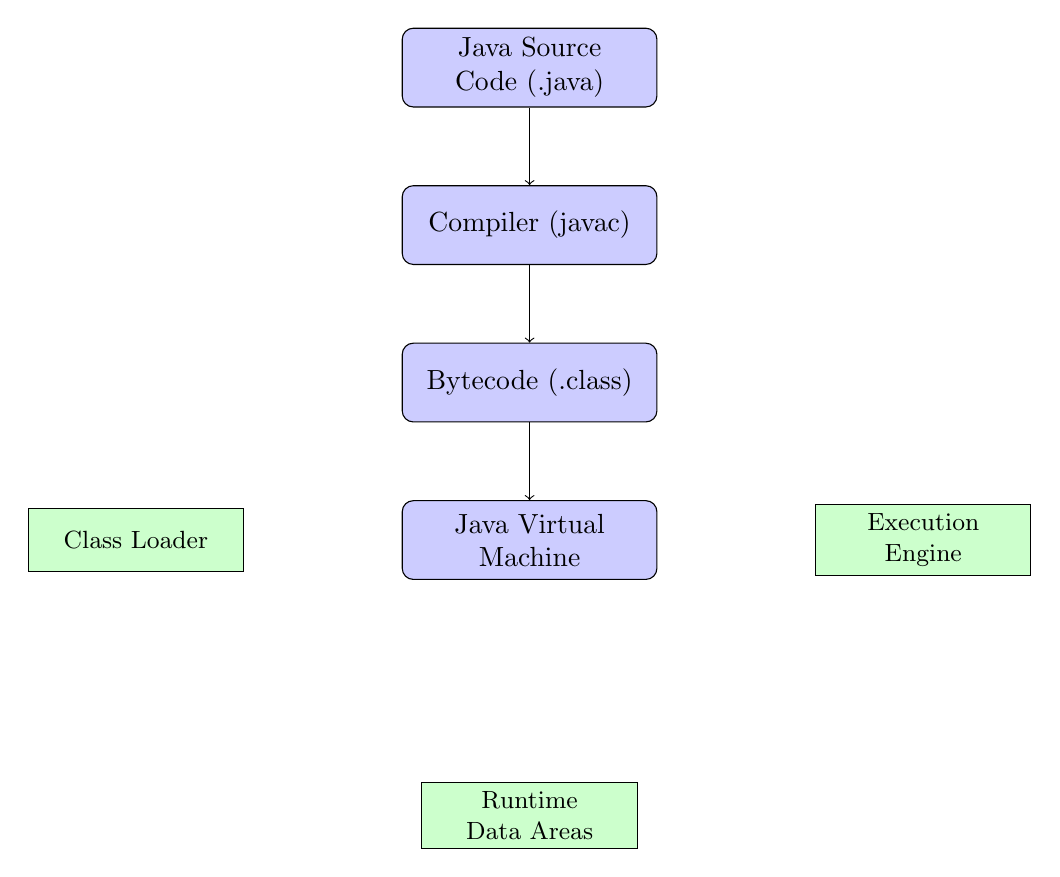
\begin{tikzpicture}[node distance=2cm, auto]
    \tikzstyle{block} = [rectangle, draw, fill=blue!20, text width=3cm, text centered, rounded corners, minimum height=1cm]
    \tikzstyle{subblock} = [rectangle, draw, fill=green!20, text width=2.5cm, text centered, minimum height=0.8cm, font=\small]
    
    \node[block] (input) {Java Source Code (.java)};
    \node[block, below of=input] (compile) {Compiler (javac)};
    \node[block, below of=compile] (bytecode) {Bytecode (.class)};
    \node[block, below of=bytecode] (jvm) {Java Virtual Machine};
    
    \node[subblock, left of=jvm, xshift=-3cm] (loader) {Class Loader};
    \node[subblock, right of=jvm, xshift=3cm] (exec) {Execution Engine};
    \node[subblock, below of=jvm, yshift=-1.5cm] (memory) {Runtime Data Areas};
    
    \draw[->] (input) -- (compile);
    \draw[->] (compile) -- (bytecode);
    \draw[->] (bytecode) -- (jvm);
    
\end{tikzpicture}
\end{center}

\subsection{Class Loader Subsystem}

The Class Loader is responsible for loading \texttt{.class} files into memory when they are first needed.

\textbf{Three phases:}

\begin{enumerate}
    \item \textbf{Loading} - Locates and reads \texttt{.class} files (Person, Student, GraduateStudent, StudentService, etc.)
    \item \textbf{Linking} - Verification of bytecode safety, preparation of memory for static variables, and resolution of symbolic references
    \item \textbf{Initialization} - Execution of static initializers and assignment of initial values to static fields
\end{enumerate}

\section{Runtime Data Areas}

The JVM defines several memory areas created when the JVM starts:

\subsection{Memory Layout Diagram}

\begin{center}
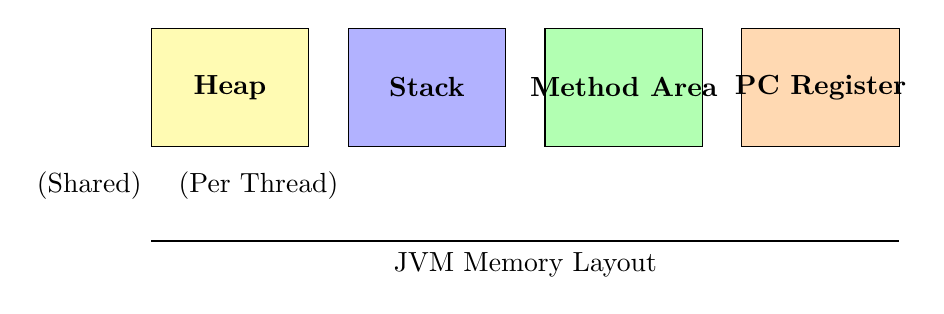
\begin{tikzpicture}
    \draw[fill=yellow!30] (0,0) rectangle (2,1.5) node[pos=.5] {\textbf{Heap}};
    \draw[fill=blue!30] (2.5,0) rectangle (4.5,1.5) node[pos=.5] {\textbf{Stack}};
    \draw[fill=green!30] (5,0) rectangle (7,1.5) node[pos=.5] {\textbf{Method Area}};
    \draw[fill=orange!30] (7.5,0) rectangle (9.5,1.5) node[pos=.5] {\textbf{PC Register}};
    
    \draw (0,-0.5) node[left] {(Shared)};
    \draw (2.5,-0.5) node[left] {(Per Thread)};
    
    \draw[thick] (0,-1.2) -- (9.5,-1.2);
    \draw (4.75,-1.5) node {JVM Memory Layout};
\end{tikzpicture}
\end{center}

\subsection{4.1 Method Area}

Stores class-level information:
\begin{itemize}
    \item Class metadata and structure
    \item Method and field information
    \item Runtime constant pool
    \item Bytecode of all methods (addStudent, displayInfo, main, etc.)
\end{itemize}

\subsection{4.2 Heap}

Shared memory for object allocation:
\begin{itemize}
    \item All \texttt{Student} and \texttt{GraduateStudent} objects
    \item \texttt{ArrayList<Student>} and \texttt{ArrayList<Course>}
    \item \texttt{Course} instances
    \item Subject to automatic garbage collection
\end{itemize}

\subsection{4.3 Java Stack}

Per-thread memory:
\begin{itemize}
    \item Stack frames for each method call
    \item Local variables (name, age, studentId, etc.)
    \item Operand stack for intermediate calculations
    \item PC (program counter) for current instruction
\end{itemize}

\subsection{Stack Frame Example}

\begin{center}
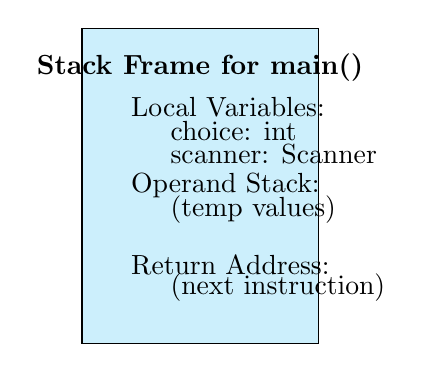
\begin{tikzpicture}
    \draw[fill=cyan!20] (0,0) rectangle (3,4);
    \draw (1.5,3.5) node {\textbf{Stack Frame for main()}};
    
    \draw (0.5,3) node[right] {Local Variables:};
    \draw (1,2.7) node[right] {choice: int};
    \draw (1,2.4) node[right] {scanner: Scanner};
    
    \draw (0.5,2) node[right] {Operand Stack:};
    \draw (1,1.7) node[right] {(temp values)};
    
    \draw (0.5,1) node[right] {Return Address:};
    \draw (1,0.7) node[right] {(next instruction)};
    
\end{tikzpicture}
\end{center}

\section{Execution Engine}

The Execution Engine reads bytecode from the Method Area and executes it.

\subsection{Interpreter vs JIT Compiler}

\begin{center}
\begin{tabular}{|l|l|l|}
\hline
\textbf{Aspect} & \textbf{Interpreter} & \textbf{JIT Compiler} \\
\hline
Startup & Fast & Slower \\
\hline
Execution Speed & Slower (line-by-line) & Fast (native code) \\
\hline
When Used & Always first & After hot spot detection \\
\hline
Code Quality & Direct bytecode & Optimized native \\
\hline
\end{tabular}
\end{center}

\subsection{Execution Flow Diagram}

\begin{center}
\begin{tikzpicture}[node distance=1.5cm]
    \tikzstyle{block} = [rectangle, draw, fill=blue!30, text width=2.5cm, text centered, minimum height=0.8cm]
    \tikzstyle{decision} = [diamond, draw, fill=yellow!30, text width=1.5cm, text centered, minimum height=0.8cm]
    
    \node[block] (load) {Load bytecode};
    \node[block, below of=load] (exec) {Execute instruction};
    \node[decision, below of=exec] (hot) {Hot spot?};
    \node[block, below of=hot, xshift=-1.5cm] (interp) {Continue Interpreting};
    \node[block, below of=hot, xshift=1.5cm] (jit) {JIT Compile};
    \node[block, below of=jit] (native) {Execute Native Code};
    
    \draw[->] (load) -- (exec);
    \draw[->] (exec) -- (hot);
    \draw[->] (hot) -- node[left] {No} (interp);
    \draw[->] (hot) -- node[right] {Yes} (jit);
    \draw[->] (jit) -- (native);
    \draw[->] (interp) -- (exec);
    \draw[->] (native) -- (exec);
    
\end{tikzpicture}
\end{center}

\section{Bytecode Execution Flow for Student Management System}

\begin{enumerate}
    \item \textbf{Compilation Phase} - \texttt{javac} compiles all \texttt{.java} files to \texttt{.class} bytecode
    \item \textbf{JVM Startup} - Command: \texttt{java com.airtribe.studentmanagement.mainpkg.StudentManagementApp}
    \item \textbf{Class Loading} - Class loader loads StudentManagementApp, then Person, Student, Course, StudentService as needed
    \item \textbf{Memory Allocation} - Runtime data areas created; Method Area stores bytecode, Heap ready for objects
    \item \textbf{Main Method Execution} - Stack frame created for main(), which calls showMenu() in a loop
    \item \textbf{User Interaction} - Each menu choice (add student, view, search, add course) creates objects on Heap
    \item \textbf{JIT Optimization} - Repeated menu operations become hot spots, JIT compiles them to native code
    \item \textbf{Garbage Collection} - When students are deleted and no references remain, Garbage Collector frees Heap memory
\end{enumerate}

\section{Diagram: Student Object Lifecycle}

\begin{center}
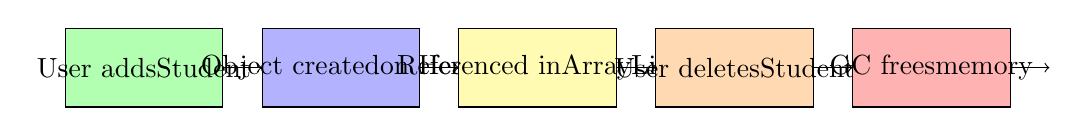
\begin{tikzpicture}
    \draw[fill=green!30] (0,0) rectangle (2,1) node[pos=.5] {User adds\\Student};
    \draw[fill=blue!30] (2.5,0) rectangle (4.5,1) node[pos=.5] {Object created\\on Heap};
    \draw[fill=yellow!30] (5,0) rectangle (7,1) node[pos=.5] {Referenced in\\ArrayList};
    \draw[fill=orange!30] (7.5,0) rectangle (9.5,1) node[pos=.5] {User deletes\\Student};
    \draw[fill=red!30] (10,0) rectangle (12,1) node[pos=.5] {GC frees\\memory};
    
    \draw[->] (2,0.5) -- (2.5,0.5);
    \draw[->] (4.5,0.5) -- (5,0.5);
    \draw[->] (7,0.5) -- (7.5,0.5);
    \draw[->] (9.5,0.5) -- (10,0.5);
    \draw[->] (12,0.5) -- (12.5,0.5);
\end{tikzpicture}
\end{center}

\section{Write Once, Run Anywhere (WORA)}

Java achieves platform independence through the WORA principle:

\begin{itemize}
    \item Source code (\texttt{.java}) is compiled into platform-independent bytecode (\texttt{.class})
    \item The same bytecode runs on any OS (Windows, Linux, macOS) with a compatible JVM
    \item The JVM abstracts hardware and OS differences, making the same compiled project portable
    \item No recompilation is needed when moving from one platform to another
\end{itemize}

\subsection{WORA Illustration}

\begin{center}
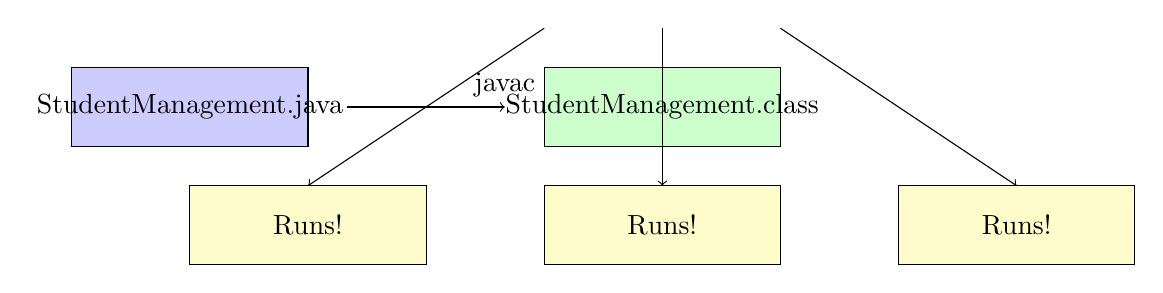
\begin{tikzpicture}
    \draw[fill=blue!20] (0,0) rectangle (3,1) node[pos=.5] {StudentManagement.java};
    \draw[->] (3.5,0.5) -- (5.5,0.5) node[above] {javac};
    \draw[fill=green!20] (6,0) rectangle (9,1) node[pos=.5] {StudentManagement.class};
    
    \draw[->] (6,1.5) -- (3,-0.5) node[below] {JVM on\\Windows};
    \draw[->] (7.5,1.5) -- (7.5,-0.5) node[below] {JVM on\\Linux};
    \draw[->] (9,1.5) -- (12,-0.5) node[below] {JVM on\\macOS};
    
    \draw[fill=yellow!20] (1.5,-1.5) rectangle (4.5,-0.5) node[pos=.5] {Runs!};
    \draw[fill=yellow!20] (6,-1.5) rectangle (9,-0.5) node[pos=.5] {Runs!};
    \draw[fill=yellow!20] (10.5,-1.5) rectangle (13.5,-0.5) node[pos=.5] {Runs!};
\end{tikzpicture}
\end{center}

\section{Key Takeaways}

\begin{itemize}
    \item The JVM provides an abstraction layer between Java code and the underlying hardware/OS
    \item Class Loader dynamically loads classes as they are needed
    \item Runtime Data Areas (Heap, Stack, Method Area) manage memory during execution
    \item The Execution Engine uses both interpretation and JIT compilation for efficient execution
    \item Garbage Collector automatically manages heap memory
    \item Java's bytecode and JVM enable true platform independence (WORA)
\end{itemize}

\end{document}
